% bei Standalone in documentclass noch:
% \RequirePackage{luatex85}

\documentclass[captions=tableheading, titlepage= firstiscover, parskip = half , bibliography=totoc]{scrartcl}
%paper = a5 für andere optinen
% titlepage= firstiscover
% bibliography=totoc für bibdateien
% parskip=half  Veränderung um Absätze zu verbessern

\usepackage{scrhack} % nach \documentclass
\usepackage[aux]{rerunfilecheck}
\usepackage{polyglossia}
\usepackage[style=numeric, backend=biber]{biblatex} % mit [style = alphabetic oder numeric] nach polyglossia
\addbibresource{lit.bib}
\setmainlanguage{german}

\usepackage[autostyle]{csquotes}
\usepackage{amsmath} % unverzichtbare Mathe-Befehle
\usepackage{amssymb} % viele Mathe-Symbole
\usepackage{mathtools} % Erweiterungen für amsmath
\usepackage{fontspec} % nach amssymb
% muss ins document: \usefonttheme{professionalfonts} % für Beamer Präsentationen
\usepackage{longtable}

\usepackage[
math-style=ISO,    % \
bold-style=ISO,    % |
sans-style=italic, % | ISO-Standard folgen
nabla=upright,     % |
partial=upright,   % /
]{unicode-math} % "Does exactly what it says on the tin."
\setmathfont{Latin Modern Math}
% \setmathfont{Tex Gyre Pagella Math} % alternativ

\usepackage[
% die folgenden 3 nur einschalten bei documenten
locale=DE,
separate-uncertainty=true, % Immer Fehler mit ±
per-mode=symbol-or-fraction, % m/s im Text, sonst \frac
]{siunitx}

% alternativ:
% per-mode=reciprocal, % m s^{-1}
% output-decimal-marker=., % . statt , für Dezimalzahlen

\usepackage[
version=4,
math-greek=default,
text-greek=default,
]{mhchem}

\usepackage[section, below]{placeins}
\usepackage{caption} % Captions schöner machen
\usepackage{graphicx}
\usepackage{grffile}
\usepackage{subcaption}

% \usepackage{showframe} Wenn man die Ramen sehen will

\usepackage{float}
\floatplacement{figure}{htbp}
\floatplacement{table}{htbp}

\usepackage{mhchem} %chemische Symbole Beispiel: \ce{^{227}_{90}Th+}


\usepackage{booktabs}

 \usepackage{microtype}
 \usepackage{xfrac}

 \usepackage{expl3}
 \usepackage{xparse}

 % \ExplSyntaxOn
 % \NewDocumentComman \I {}  %Befehl\I definieren, keine Argumente
 % {
 %    \symup{i}              %Ergebnis von \I
 % }
 % \ExplSyntaxOff

 \usepackage{pdflscape}
 \usepackage{mleftright}

 % Mit dem mathtools-Befehl \DeclarePairedDelimiter können Befehle erzeugen werden,
 % die Symbole um Ausdrücke setzen.
 % \DeclarePairedDelimiter{\abs}{\lvert}{\rvert}
 % \DeclarePairedDelimiter{\norm}{\lVert}{\rVert}
 % in Mathe:
 %\abs{x} \abs*{\frac{1}{x}}
 %\norm{\symbf{y}}

 % Für Physik IV und Quantenmechanik
 \DeclarePairedDelimiter{\bra}{\langle}{\rvert}
 \DeclarePairedDelimiter{\ket}{\lvert}{\rangle}
 % <name> <#arguments> <left> <right> <body>
 \DeclarePairedDelimiterX{\braket}[2]{\langle}{\rangle}{
 #1 \delimsize| #2
 }

\setlength{\delimitershortfall}{-1sp}

 \usepackage{tikz}
 \usepackage{tikz-feynman}

 \usepackage{csvsimple}
 % Tabellen mit \csvautobooktabular{"file"}
 % muss in table umgebung gesetzt werden


% \multicolumn{#Spalten}{Ausrichtung}{Inhalt}

\usepackage{hyperref}
\usepackage{bookmark}
\usepackage[shortcuts]{extdash} %nach hyperref, bookmark

\newcommand{\ua}[1]{_\symup{#1}}
\newcommand{\su}[1]{\symup{#1}}


\title{Versuch 355}
\subtitle{Gekoppelte Schwingkreise}
\author{Sebastian Pape\\
        sepa@gmx.de \and
        Jonah Nitschke\\
        lejonah@web.de}
\date{Durchführung: 10.01.2017\\
      Abgabe: 17.01.2017}

\begin{document}
\maketitle
\setcounter{page}{1}

\section{Theorie}

\section{Zielsetzung}

In dem Versuch V355 werden gekoppelte schwingfähige Systeme in Form von elektrischen
Schaltungen betrachtet. Vom besonderem Interesse sind hierbei der stattfindende
Energieaustausch zwischen den Systemen, sowie die Schwingungsfrequenzen.
Es werden elektrische Schaltungen betrachtet, da die Amplituden und Frequenzen
der Schwingungen besonders präzise gemessen und beobachtet werden.

\subsection{Gekoppelte Schwingungen}

Als eine Schwingungen wird ein Forgang bezeichnet, bei dem ein System periodisch
zwischen zwei Zuständen wechselt. Werden zwei schwingende Systeme gekoppelt,
wechselwirken diese miteinander. Die Wechselwirkung wird in Form von einem
Energiaustausch zwischen den Systeme vollzogen. In dem Versuch wurden zwei identische
Schwingkreise über einen Kopplungskondensator $C_K$ gekopplet. Eine schematische
Darstellung eines gekoppelten elektrischen Schwingkreises ist in der Abb.
\ref{fig:gekoppelterSchwingkreis} dargestellt.

\begin{figure}
  \centering
  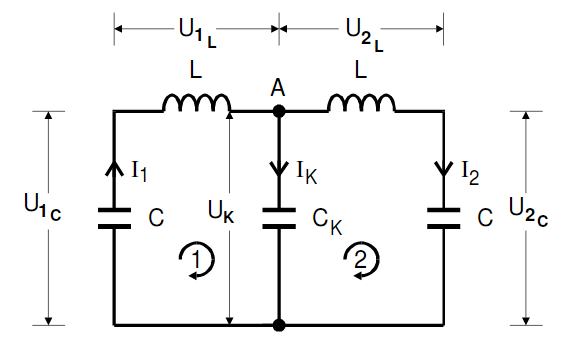
\includegraphics[width=9cm]{V355_allg_Schwingkreis.png}
  \caption{Gekoppelter elektrischer Schwingkreis.\cite{anleitung01}\protect}
  \label{fig:gekoppelterSchwingkreis}
\end{figure}

Über die Kirchhoffschen Regelen und Differentiation lassen sie die folgenden
Schwingungsgleichugen aufstellen.

\begin{align}
  \label{eqn:DGL_1}
  L\ddot{I_1} + \frac{1}{C}I_1+\frac{1}{C_K}\left(I_1 - I_2 \right) &= 0\\
  \label{eqn:DGL_2}
  L\ddot{I_2} + \frac{1}{C}I_2-\frac{1}{C_K}\left(I_1 - I_2 \right) &= 0
\end{align}

Über Addition und Subtraktion werden \eqref{eqn:DGL_1} und \eqref{eqn:DGL_2}
zu:

\begin{align}
  \label{eqn:DGL_1+2}
  L\left(\ddot{I_1} + \ddot{I_2}\right) + \frac{1}{C}\left(I_1 + I_2\right)&=0\\
  \label{eqn:DGL_1-2}
  L\left(\ddot{I_1} - \ddot{I_2}\right) + \left(\frac{1}{C} + \frac{2}{C_K}\right)\left(I_1 - I_2\right)&=0.
\end{align}

Die Lösung von \eqref{eqn:DGL_1+2} ist eine Schwingungsgleichung mit der Frequenz
\begin{equation}
  \nu^+ = \frac{1}{2\pi\sqrt{LC}}.
\end{equation}
Die DGL \eqref{eqn:DGL_1-2} ist ebenfalls
lösbar durch eine Schwingungsgleichung. Die Lösung hat eine Frequenz von
\begin{equation}
  \nu^- = \frac{1}{\left[2\pi\sqrt{L\left(\frac{1}{C}+\frac{2}{C_K}\right)^{(-1)}}\right]}.
\end{equation}
Die Lösungen haben die Form:

\begin{align}
  \left(I_1 + I_2\right)(t) &= \left(I_{1,0} + I_{2,0}\right)cos\left(2\pi\nu^+t\right)\\
  \left(I_1 - I_2\right)(t) &= \left(I_{1,0} - I_{2,0}\right)cos\left(2\pi\nu^-t\right).
\end{align}

Die ermittelten Frequenzen $\nu^+$ und $\nu^-$ heißen Fundamentalfrequenzen,
da sie die Frequenzen der Fundamentalschwingungen sind. Als Fundamentalschwingungen
werden die Spezialfälle der Schwingungen eines gekoppelten Systems bezeichnet.
Der erste Spezialfall ist, wenn die beiden Oszillatoren mit der selben
Amplitude und Frequenz schwingen.
In diesem Fall ist die Kopplung minimal, da die Systeme nicht miteinander interargieren
und es liegt die Frequenz $\nu^+$ vor. Der andere Spezialfall beschreibt die
gegenphasige Schwingung bei gleicher Amplitude der Systeme. In diesem Fall
ist die Kopplung maximal und es liegt die Frequenz $\nu^-$ vor.

\subsubsection{Schwebungen}

Bei den Fundamentalschwingungen waren beide Oszillatoren bei Betrachtungsanfang
gleich- bzw. gegenphasig. Es treten von den Fundamentalschwingungen
verschiedene Schwingverhalten auf, wenn einer der Oszillatoren bei
Beobachtungsbeginn z.B. in Ruhe ist.
Das dann auftretende Schwingverhalten wird als Schwebung bezeichnet.
Dieses Schwingverhalten lässt sich durch die folgenden Gleichungen beschreiben.

\begin{align}
  \label{eqn:Schwebung_1}
  I_1(t) = I_{1,0}cos\left(\frac{1}{2}\left(\omega^+ + \omega^-\right)t\right)cos\left(\frac{1}{2}\left(\omega^+-\omega^-\right)t\right)\\
  \label{eqn:Schwebung_2}
  I_2(t) = I_{1,0}sin\left(\frac{1}{2}\left(\omega^+ + \omega^-\right)t\right)sin\left(\frac{1}{2}\left(\omega^+-\omega^-\right)t\right)
\end{align}

Dabei ist $\omega^+ = 2\pi\nu^+$ und $\omega^- = 2\pi\nu^-$.
Unter der Annahme, dass die Fundamentalschwingungen $\nu^+$ und $\nu^-$ ungefähr
gleich sind gilt:$\frac{1}{2}\omega^++\omega^-\approx\omega^+$, sowie
$\omega^- + \omega^+ \ll\omega^+$.
In den Gleichungen \eqref{eqn:Schwebung_1} und \eqref{eqn:Schwebung_2} wird
ersichtlich, dass unter der getroffenen Annahme der erste Faktor in den Gleichungen
ungefähr mit der Einzelschwingung eines entkoppelten Oszillators übereinstimmt.
Der Zweite Faktor beschreibt ebenfalls eine Schwingung mit einer Frequenz
$\ll\omega^+$. Dies ist der Schwebungsanteil der Schwingung.
Die Differenz der Fundamentalschwingungen wird als Schwebungsfrequenz
bezeichnet. Die Abbildung \ref{fig:Schwebung} zeigt ein exemplarische Darstellung
einer Schwebung.

\begin{figure}
  \centering
  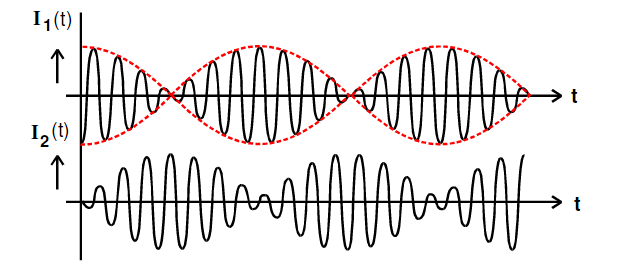
\includegraphics[width=9cm]{V355_Schwebung.png}
  \caption{Beispiel einer Schwebung.\cite{anleitung01}\protect}
  \label{fig:Schwebung}
\end{figure}

\end{document}
